\section{\textbf{Wait-Free Snapshots}}
% ---------------------------------------------------------------------------- %
\subsection{Particular Case}
\par
In this experiment we are dealing with the problem of creating an algorithm to
create a Snapshot of a set of Register in such a way that the algorithm
garantees a Wait-Free operation.
\par
% ---------------------------------------------------------------------------- %
\subsection{Solution}
\par
The purpose of a Wait-Free snapshot is to overcome the problems of the Simple snapshot presented before. Let us remember that such snapshot executes sucesive collect() operations. Once it achieves a \textit{clean double collect}, it returns the snapshot. Otherwise, it keeps trying. 
\par
One of the ideas behind the Wait-Free Snapshot is that when a double collect fails, it is because a update interfered. That means that the updater could take a snapshot right before its update and other threads could use it as their snapshot too. 
\par
% ---------------------------------------------------------------------------- %
\subsection{Experiment Description}
\par
In this experiment, the test looks a bit different. Let us explain how it is
different. In this case we have two experiments:
\par
\begin{enumerate}
\item testSequential. We spawn a new thread that updates the register with a
value of \textit{FIRST} and right after that, it scans the value of the
register. The expected result is that this read retrieves the value of
\textit{FIRST}
\item testParallel. We spawn \textit{THREADS} number of threads (in our case it
is $2$). Each of them will first update its register with a value of
\textit{FIRST} and then with a value of \textit{SECOND}. Each thread then
updates a position in a matrix of size \textit{THREADS}$x$\textit{THREADS} with
the result of doing a $scan()$ operation. At the end we compare consecutive rows
in the matrix. The comparison is done entry by entry and we should see that for
some entries the first entry is greater and for some others it is smaller than
the second. What we must see is that some times the first entry is that all
entries are equal and we allow the first to sometimes be either greater or
smaller than the second one.
\end{enumerate}
\par
These are the details of the system we used to run the experiments:
\begin{itemize}
\item Processor: Intel Core i5 @2.5 GHz. 2 Cores.
\item L2 Cache per Core: 256 KB
\item L3 Cache: 3 MB
\item System Memory: 16 GB
\end{itemize}
% ---------------------------------------------------------------------------- %
\subsection{Sample Results}
\par
For this test, we saw that in every try, both test cases passed.
\par
\begin{figure}[h]
  \centering
  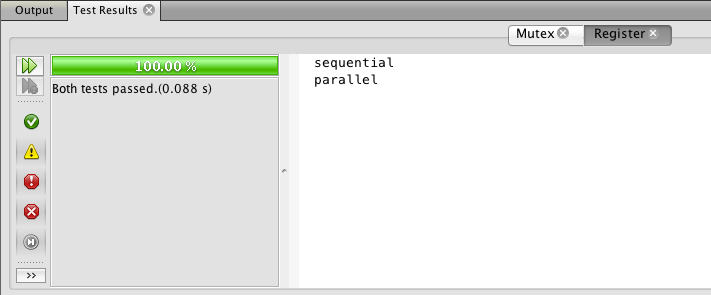
\includegraphics[width=13cm]{WFS00.png}
  \caption{Successful execution of the tests for Wait-Free Snapshot}
  \label{fig:WFS00}
\end{figure}
\par
\begin{figure}[h]
  \centering
  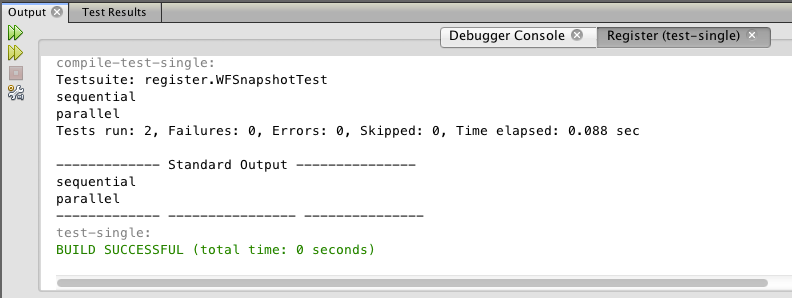
\includegraphics[width=13cm]{WFS01.png}
  \caption{Successful execution of the tests for Wait-Free Snapshot}
  \label{fig:WFS01}
\end{figure}
\par
% ---------------------------------------------------------------------------- %
\subsection{Interpretation}
% ---------------------------------------------------------------------------- %
In this experiment we were able to observe how a Wait-Free Snapshot can be
constructed. 
